Published in The Astrophysical Journal Letters \citep{calcino2022} and publicly available at \href{https://arxiv.org/abs/2111.07416v2}{\url{arXiv:2111.07416v2}}.

\subsubsection{Abstract}

We map the planetary wake associated with the embedded protoplanet creating the CO kink in the disk of HD~163296. We show that the wake can be traced by a series of correlated perturbations in the peak velocity map. The sign change of the perturbations across the disk major axis confirm that the wake induces predominantly radial motion, as predicted by models of planet-disk interaction. These results provide the first direct confirmation of planet wakes generated by Lindblad resonances. Mapping the wake provides a constraint on the disk aspect ratio, which is required to measure the mass of the planet.

\section{Introduction}

The protoplanetary disk of HD~163296 has been shown to contain kinematic signatures associated with a perturbing planet \citep{pinte2018a,teague2018}.
Millimetre continuum and CO spectral line observations taken at high spatial resolution have revealed additional substructures in both the DSHARP \citep{andrews2018,huang2018b,pinte2020,izquierdo2021} and MAPS \citep{oberg2021,teague2021} large programs using ALMA.
Spiral features have been identified in kinematics, in both channel maps and velocity residuals \citep{teague2021}.
The so-called \textit{velocity kinks} found in the velocity channel maps arise from perturbations in the bulk gas motions, causing modifications to the line-of-sight velocity field.
Specifically, we define a velocity kinks as a localised distortion of the iso-velocity curve caused by deviations from Keplerian motion, shifting line emission into an adjacent channel.
Perturbations that cause kinks may be caused by spiral density waves induced by either gravitating bodes such as planets, or the gravitational instability mechanism \citep{hall2020}.
The velocity kinks detected in CO emission observations of HD~163296 have been associated with an embedded planet \citep{pinte2018a}.

In \citet{bollati2021} (hereafter \citetalias{bollati2021}), we developed a semi-analytic framework for predicting velocity kinks caused by the planet-disk interaction, using the mathematical theory of density waves launched at the Lindblad resonances by tidal forcing \citep{goldreich1979,goldreich1980,goodman2001,ogilvie2002,rafikov2002a}.
Applying this model to the kinematic planet detection in HD~163296 by \citet{pinte2018a} we can interpret velocity kinks as occurring whenever the planet wake ``crosses'' a velocity channel present in the data.
The analytics therefore predict that kinks should extend throughout the disk, including far from the planet (see Figure~\ref{fig:2D_kinks}).
The non-localised \textit{secondary kinks} induced far from the planet should be detectable, but have thus far not been seen in kinematic observations.
In \citetalias{bollati2021} we tried to reconcile this apparent conflict by supposing that either secondary kinks are washed out by the finite beam size, or that perhaps they are suppressed through viscous damping of the planet wake.
The high spatial resolution MAPS data means that the former hypothesis is no longer tenable.

In this letter we show that secondary kinks \textit{are} observed in the kinematic MAPS data of HD~163296, and that they may be used to trace the spiral planet wake over a large fraction of the disk.
Specifically, the wake may be mapped through spatially correlated features in the peak velocity map given sufficient spatial and spectral resolution.
Determining the shape of the planet wake also constrains the temperature structure of the disk, which is necessary for planet mass recovery through measuring velocity kink amplitudes \citepalias{bollati2021}.

\section{Methods}

\subsection{Observations}

We used the JvM corrected \citep{jorsater1995} $^{12}$CO $J=2-1$ \textit{robust=0.5} line emission observations of HD~163296 from the MAPS large program (2018.1.01055.L, \citealt{oberg2021,czekala2021})\footnote{The data are available for download at \url{http://alma-maps.info/}.}.
The beam size of the observations is approximately $0.14" \times 0.11"$, the position angle is $104^\circ$, the spectral resolution is $92 \, \mathrm{m/s}$ and the channels spacing is $200 \mathrm{m/s}$.
The data is identical to that used by \citet{teague2021} in their study of the kinematics of HD~163296.
We assumed a systemic velocity velocity of  $v_{\textrm{los}}= 5.76$ km/s \citep{teague2021}.

\citet{law2021a} fit the following parameterisation to the CO emitting surface of the disk
\begin{align}
    z(r) = z_0 \left( \frac{r}{1"} \right)^\phi \exp \left( -\left[ \frac{r}{r_\mathrm{taper}} \right]^{\psi} \right), \label{eq:height}
\end{align}
following the method developed by \citet{pinte2018}, which encodes a flaring structure with an exponential taper.
They found best-fitting parameters of $z_0 = 0.388$, $\phi = 1.851$, $r_\textrm{taper} = 2.362"$, and $\psi = 1.182$, which we adopt for calculating the CO emitting layer.

\subsection{Hydrodynamical Modelling} \label{sec:calcino_hydro}

We simulated the interaction of a gas disk and an embedded 3 M$_\textrm{J}$ in 3D using the SPH code \textsc{phantom} \citep{price2018}.
We used two million SPH particles to model a disk of mass $10^{-2} \, \mathrm{M_\odot}$ surrounding a $1.9 \, \mathrm{M_\odot}$ star.
The planet and star were both modelled as sink particles \citep{bate1995}, with accretion radii of $5$ au and $5.56 \, \mathrm{au} = r_{\rm H}/4$ respectively, where $r_{\rm H}$ is the Hill radius of the planet \citep{hill1878}.
The SPH particles were initialised according to the surface density profile
\begin{align}
    \Sigma (r) \propto \left(\frac{r}{r_\mathrm{p,i}}\right)^{-p} \exp \left[-\left(\frac{r}{r_{\rm c}}\right)^{2-p}\right], \label{eq:sigma_phantom}
\end{align}
where $r_\textrm{p,i} = 280$ au is the initial location of the planet, $p = 1$, and  $r_{\rm c} = 100 $ au.
We assumed the disk to be locally isothermal choosing $c_\textrm{s} \propto (r/r_\textrm{p,i})^{-q}$ with $q = 0.35$.
These parameters were all set following \citet{pinte2018a}, except that $r_{\rm p,i}$ was increased to allow for migration.
We took the aspect ratio to be $(H/r)_{\textrm{p,i}} = 0.1$ as in \citet{degregorio-monsalvo2013} and \citet{pinte2018a}.
The simulation was evolved for 50 complete orbits of the planet, during which time the planet migrated inwards to a radius of $r_p = 256$ au, where the disk aspect ratio was slightly smaller $h_p/r_p \sim 0.09$.
The final mass of the planet was $\sim 4$ $\mathrm{M_J}$.

The simulations results were passed to the radiation transfer code \textsc{mcfost} \citep{pinte2006,pinte2009} to generate synthetic CO observations.
We included dust as a fixed ratio of $1/100$ times the gas content from the simulation, and adopted a grain size distribution of $dn(a) \propto a^{-3.5} \, da$ including spherical grains in the range  $0.03 \, \mu$m -- $1$ mm with a silicate composition \citep{weingartner2001}.
We set the effective surface temperature and radius of the star to $T_\textrm{eff} = 9250$ K and $R_\star = 1.6 $ $\mathrm{R_\odot}$ respectively, resulting in a luminosity of $\sim 17$ L$_\odot$ \citep{setterholm2018}.

\begin{figure}[H]
    \centering
    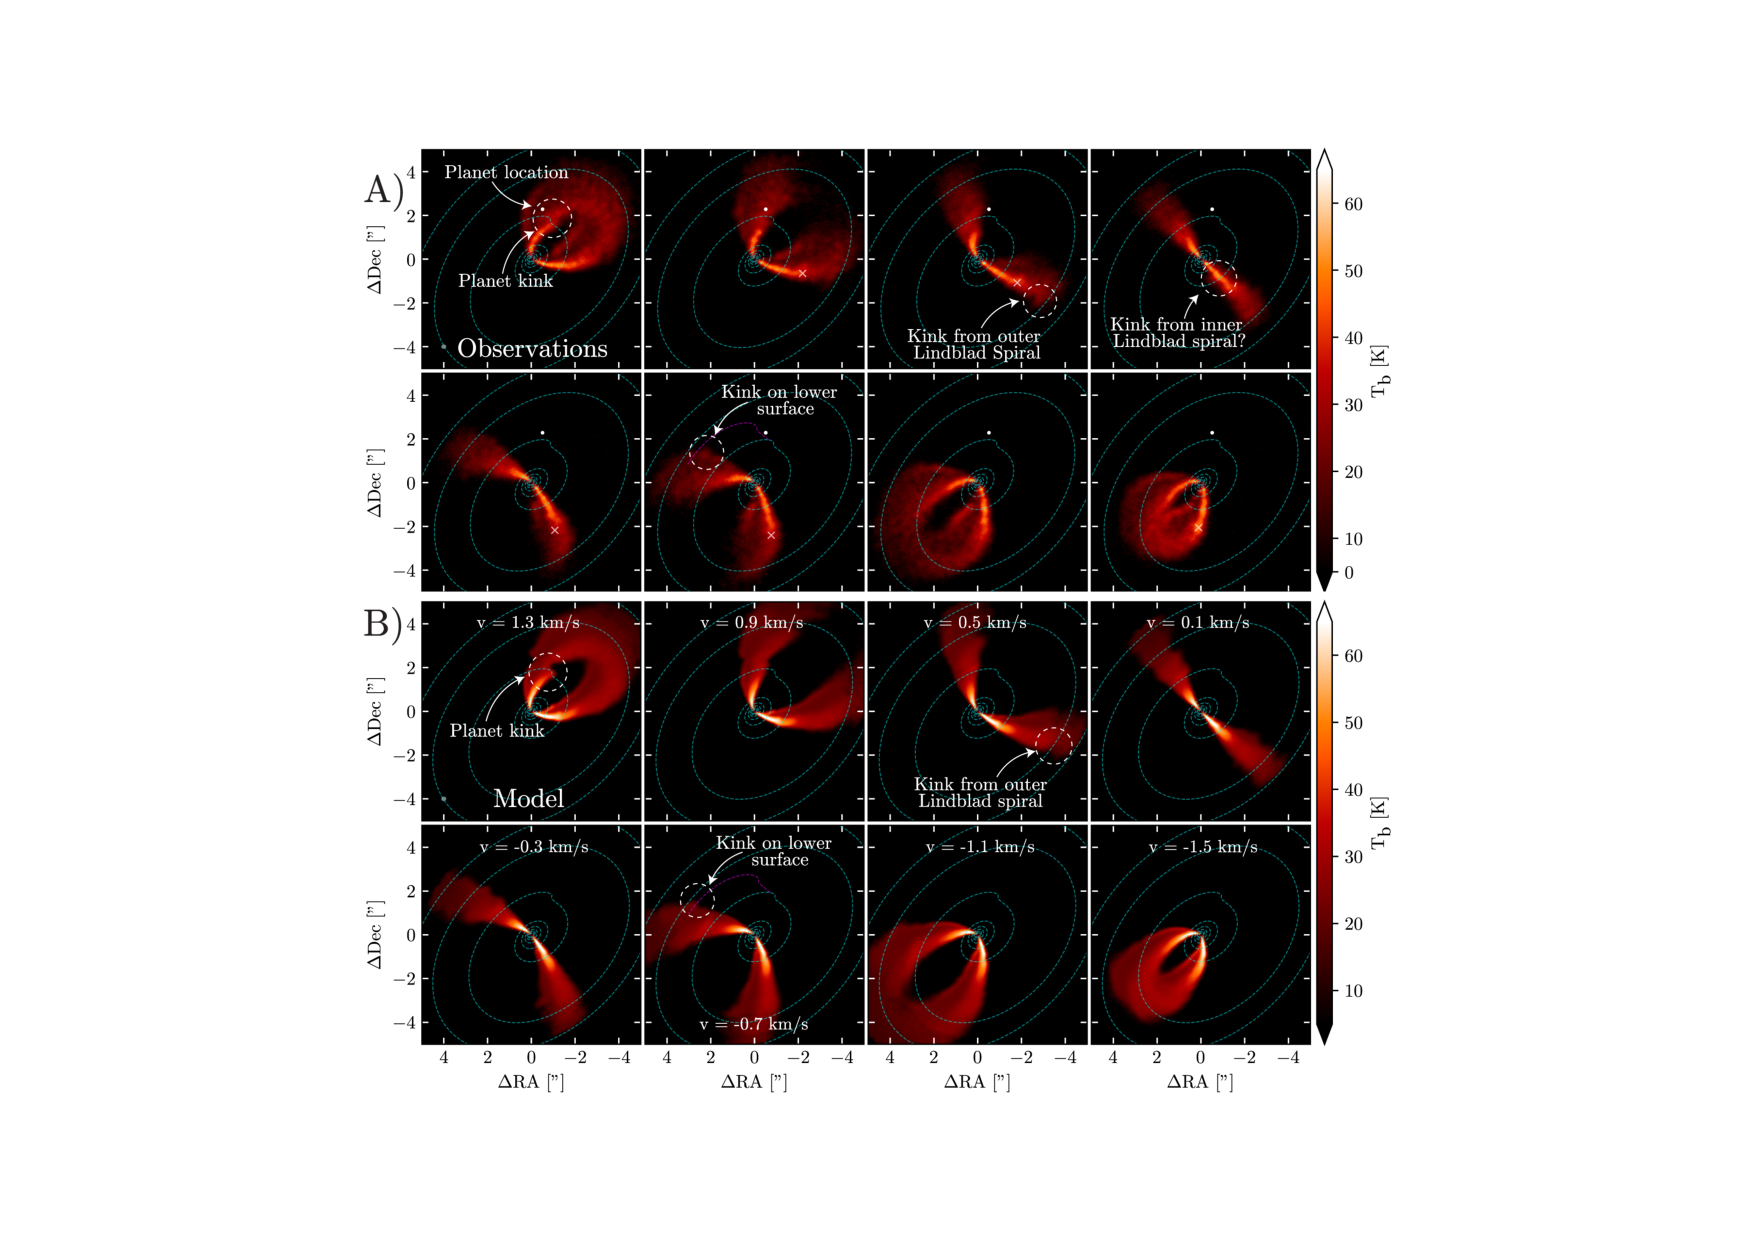
\includegraphics[width = 0.99\textwidth]{figures/calcino_sims.pdf}
    \caption{Subplot A shows velocity channels from the $^{12}$CO $J=2-1$ spectral line emission observed in the disk of HD~163296 \citep{oberg2021}. Subplot B shows the same channels from our synthetic observations generated from the SPH model. Also plotted is the location of the spiral planet wake (cyan dashed line) on the top emission surface, to demonstrate that it is co-located with the kinks present in both the observations and the simulation. The magenta line in panel two of the second row gives the wake location on the bottom emission surface. Opaque crosses mark additional kinematic features not associated with the planet wake.}
    \label{fig:calcino_channels}
\end{figure}

The central star was modelled as an isotropically radiating blackbody, and $10^8$ photon packets were used to compute temperature structure.
We assumed equal dust and gas temperatures, as well as local thermodynamic equilibrium.
The CO abundance ratio was taken to be $^{12}$CO/H$_2 = 5\times 10^{-5}$, and the effects of CO freeze-out at $T < 20\, \mathrm{K}$, and photodissociation and photodesorption in regions of high UV were included following Appendix B of \citet{pinte2018}.

We created synthetic velocity channels for the $^{12}$CO $J=2-1$ transition, with a channel spacing of $20 \, \mathrm{m/s}$.
This was then linearly interpolated over 5 channels and averaged after spectral convolution with the Hanning function, resulting in a channel width of $100 \, \mathrm{m/s}$ and spacing of $200 \, \mathrm{m/s}$.
The images were then spatially convolved with a Gaussian of width $0.15"$ to replicate the beam size in the observations.

%This difference in mass compared to the analytics is not significant, being smaller than the measurement error from kinematics at present \citep[e.g.][]{pinte2018}.

\subsection{Spiral Wake Mapping and Analytical Modelling}

\begin{figure}
    \centering
    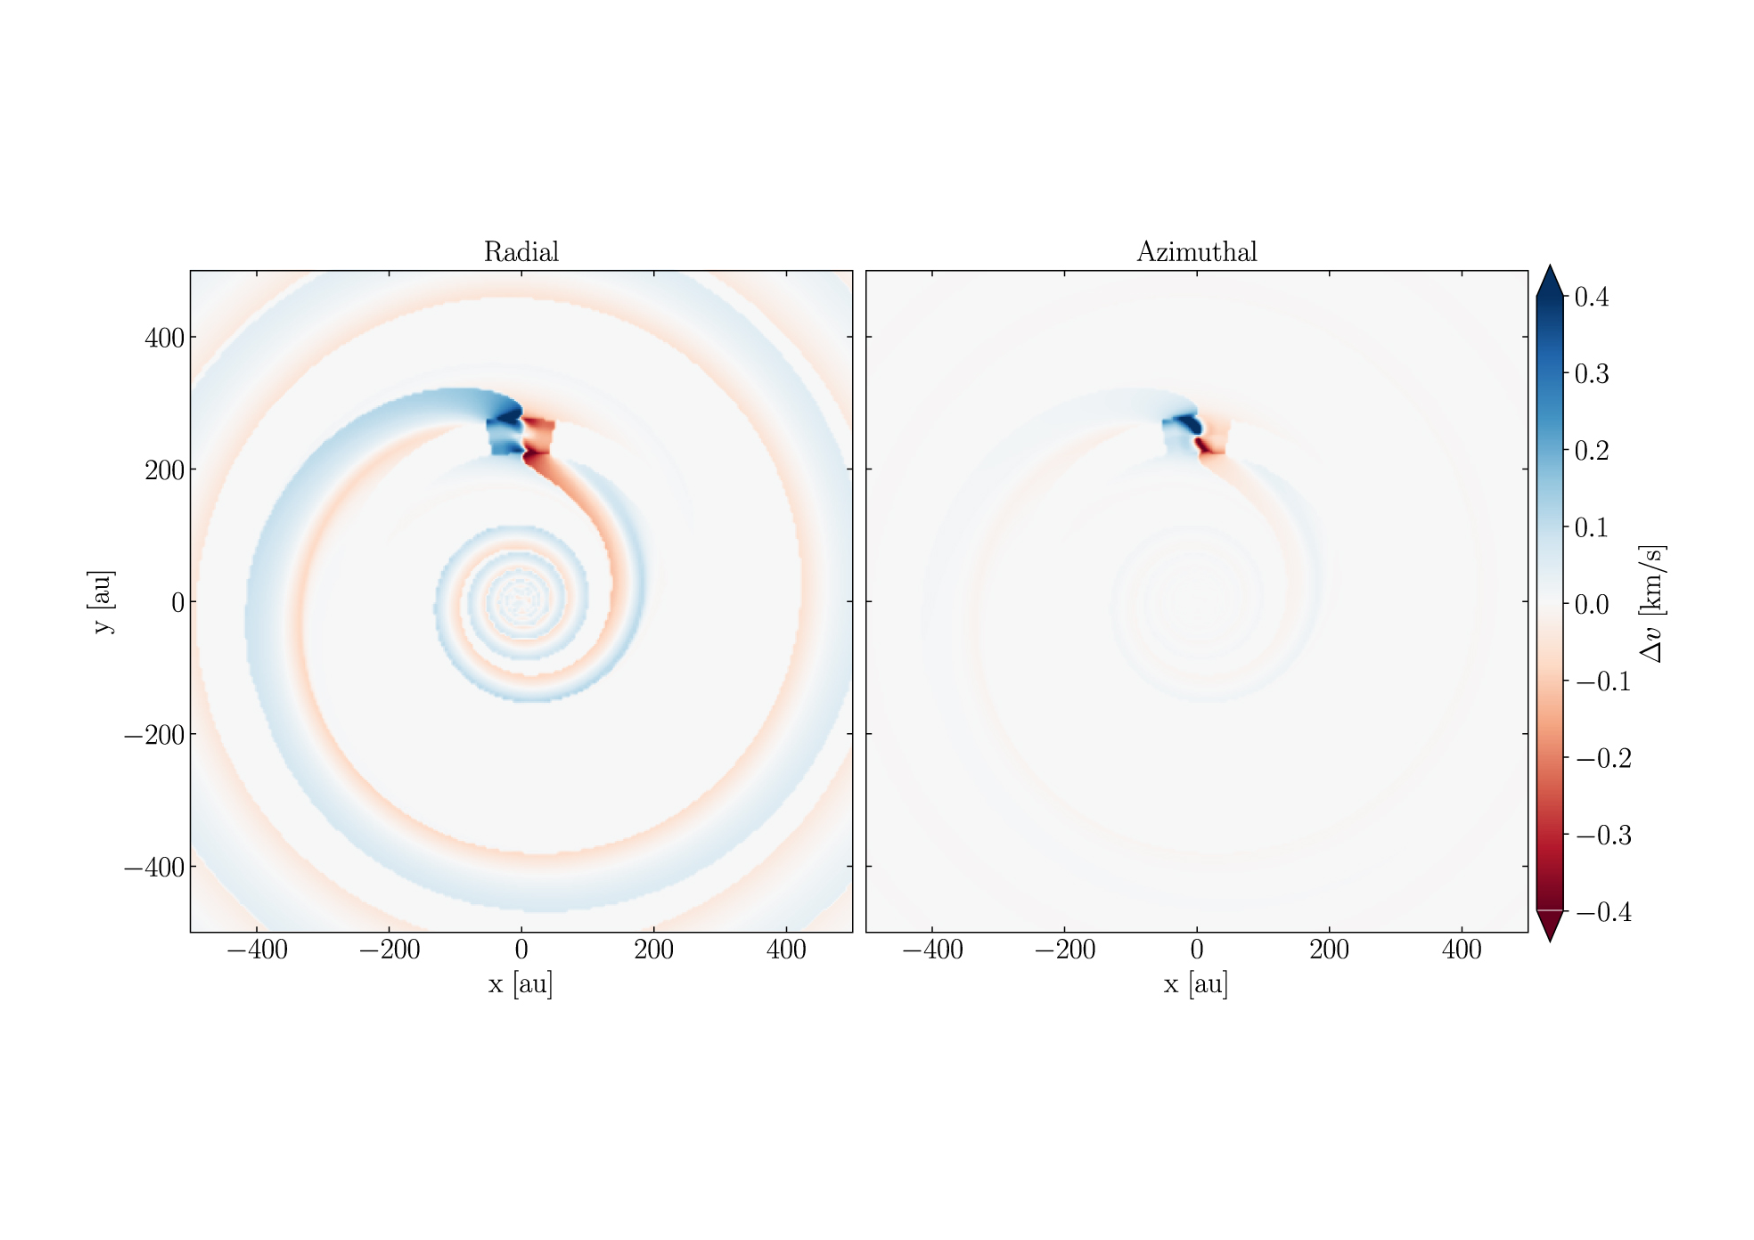
\includegraphics[width = 0.99\textwidth]{figures/calcino_analytics.pdf}
    \caption{Radial (left) and azimuthal (right) components of the velocity perturbations in the semi-analytic model, due to a $3\, \mathrm{M_J}$ planet with orbital radius $250$ au, where $(H/r)_{\rm p}=0.08$. For the radial components the positive direction is associated with increasing distance from the centre star, while the positive direction of the azimuthal components is defined such that the disk rotates in the positive direction.}
    \label{fig:calcino_analytics}
\end{figure}

Assuming a Keplerian power law disk we calculated the wake shape by \citep{rafikov2002a}
\begin{align}
    \phi_{\rm wake}(r) = \phi_{\rm p} + {\rm sgn} \left( r - r_{\rm p} \right) \frac{r_{\rm p}}{H_{\rm p}} \left[ \frac{2}{2q-1} \left(\frac{r}{r_{\rm p}}\right)^{q-\frac{1}{2}} - \frac{1}{q+1} \left(\frac{r}{r_{\rm p}}\right)^{q+1} - \frac{3}{\left(2q-1\right)\left(q+1\right)} \right], \label{eq:power_law_wake}
\end{align}
as described in section \ref{sec:transformations}, where $q$ is the sound speed index $c \propto r^{-q}$.
We initially took $q=0.35$ and $(H/r)_{\rm p}=0.09$ as in the SPH model, but we found that adjusting the aspect ratio slightly to $(H/r)_{\rm p}=0.08$ resulted in a better match between the wake and the prominent kink on the south side of the disk.

We generated a semi-analytic model with \textsc{wakeflow}, adopting the same parameters as the simulation except for the aspect ratio as mentioned, and we also used a slightly less massive planet of $3 \, \mathrm{M_J}$\footnote{This difference in mass was chosen deliberately to adjust for the change in the mass unit as a result of the slightly modified $(H/r)_{\rm p}$. From equation \ref{eq:thermalmass} we see that the relevant mass unit for planet-induced perturbations scales as $M_{\rm th} \propto (H/r)_{\rm p}^3$, and so the $\sim 11 \%$ reduction in aspect ratio results in a mass unit $\sim 30 \%$ smaller, hence the choice of $3 \, \mathrm{M_J}$ instead of $4 \, \mathrm{M_J}$ in the analytic model.}.
We used a $500 \times 500$ grid for the analytic model, and took the solution only in the mid-plane.
Note that the background disk model \ref{eq:omega_wf_ps} includes the correction due to gas pressure support.

We then projected both the wake shape and the velocities of the analytic model to the CO emitting layer given by equation \ref{eq:height}, assuming that the velocity perturbations are independent of height.
The wake and velocity fields were then rotated to match the disk inclination of $i=46^{\circ}$ and PA of $313^{\circ}$.
This allowed us to find both the shape of the wake on the sky plane and the line-of-sight velocities resulting from the planet-induced perturbations.
The projection assumes that the disk is locally isothermal since $c$ is assumed to be independent of height, just as in the SPH simulations.
In reality the temperature structure is vertically stratified \citep{calahan2021}, which may cause the pitch angle of the spiral arms to increase in the upper layers (see section \ref{sec:limitations})

\section{Results}

Figure~\ref{fig:calcino_channels} shows a comparison of the observed CO channels with the corresponding channels from the hydrodynamical model, with annotations highlighting several features.
We also plot on each Figure~the shape of the planet wake predicted by equation \ref{eq:power_law_wake} and projected to the top emitting CO surface of the disk (equation \ref{eq:height}).
The top left panel shows the original velocity kink found by \citep{pinte2018a} that is associated with the embedded planet.
However, in the third panel of the top row we highlight an additional velocity kink on the opposite side of the disk to the planet and at a larger radial separation from the star.
This feature is also seen in the SPH model (see the third panel of the third row), and is caused by the outer planet wake.
Interestingly this feature was actually predicted in \citep{pinte2018a} and can be seen in their Figure~5.
The kink can also be seen in their observations, but it was unnoticed at the time.

In the second panel of the second row of Figure~\ref{fig:calcino_channels} we have also pointed out a faint kink on the lower disk surface, which is also seen in the SPH model (row 4 panel 2).
This feature is also due to the outer wake, and to highlight this we have plotted the wake shape projected to the lower disk surface (magenta dashed line).
An associated kink on the top surface is also seen in the simulation, but is hard to make out in the observations due to the low contrast in that part of the image.

We have highlighted additional kinks present in the channel maps with opaque crosses.
These do not seem to be associated with the planet wake, but are still spatially correlated in nearby channels (see panels 2 and 3 of row 1, and panels 1 and 2 of row 2), suggesting that they are part of some extended feature.
They also do not seem to be present in the simulation.

The height of the CO emitting layer is discrepant between our simulated model and the observations.
Increasing the aspect ratio of the disk would help account for this, but would also result in a larger pitch angle for the outer spiral arm.
This behaviour likely comes down to the difference in temperature structure between the SPH simulation and the radiation transfer performed with \textsc{mcfost}.
In the former the temperature is a prescribed function of radius, while in the latter it is computed self-consistently.
Resolving this issue will require a more accurate treatment of the temperature structure in the SPH simulation, which will alter the emission layer and the wave propagation.
Further implications of this are discussed in section~\ref{sec:limitations}.

The mid-plane velocity perturbations for the analytic model are shown in Figure~\ref{fig:calcino_analytics}.
The left and right panel show the radial and azimuthal components of the velocity perturbations respectively.
From this we can see that, except for very close to the planet where the components are comparable, the azimuthal perturbations are almost negligible and the radial component certainly dominates the overall perturbation.
In the analytic model this is a feature baked into the non-linear evolution due to the local nature of the solution under the WKB approximation (see section~\ref{sec:nonlinear_evolution} for further detail), however the behaviour is also seen in the supplementary material of \citet{pinte2019} where the global non-linear behaviour is accounted for.

The thermal mass for the analytic solution is $M_{\rm th} \approx 1.5 \, \mathrm{M_J}$, and so the $3 \, \mathrm{M_J}$ planet corresponds to $\sim 2 \, M_{\rm th}$.
We are therefore in the high mass regime where the linear solution fails, resulting in the overestimation of perturbation nearby the planet, and in discontinuities at the edge of the linear box.
These discontinuities are clearly seen in Figure~\ref{fig:calcino_analytics}.

\begin{figure}
    \centering
    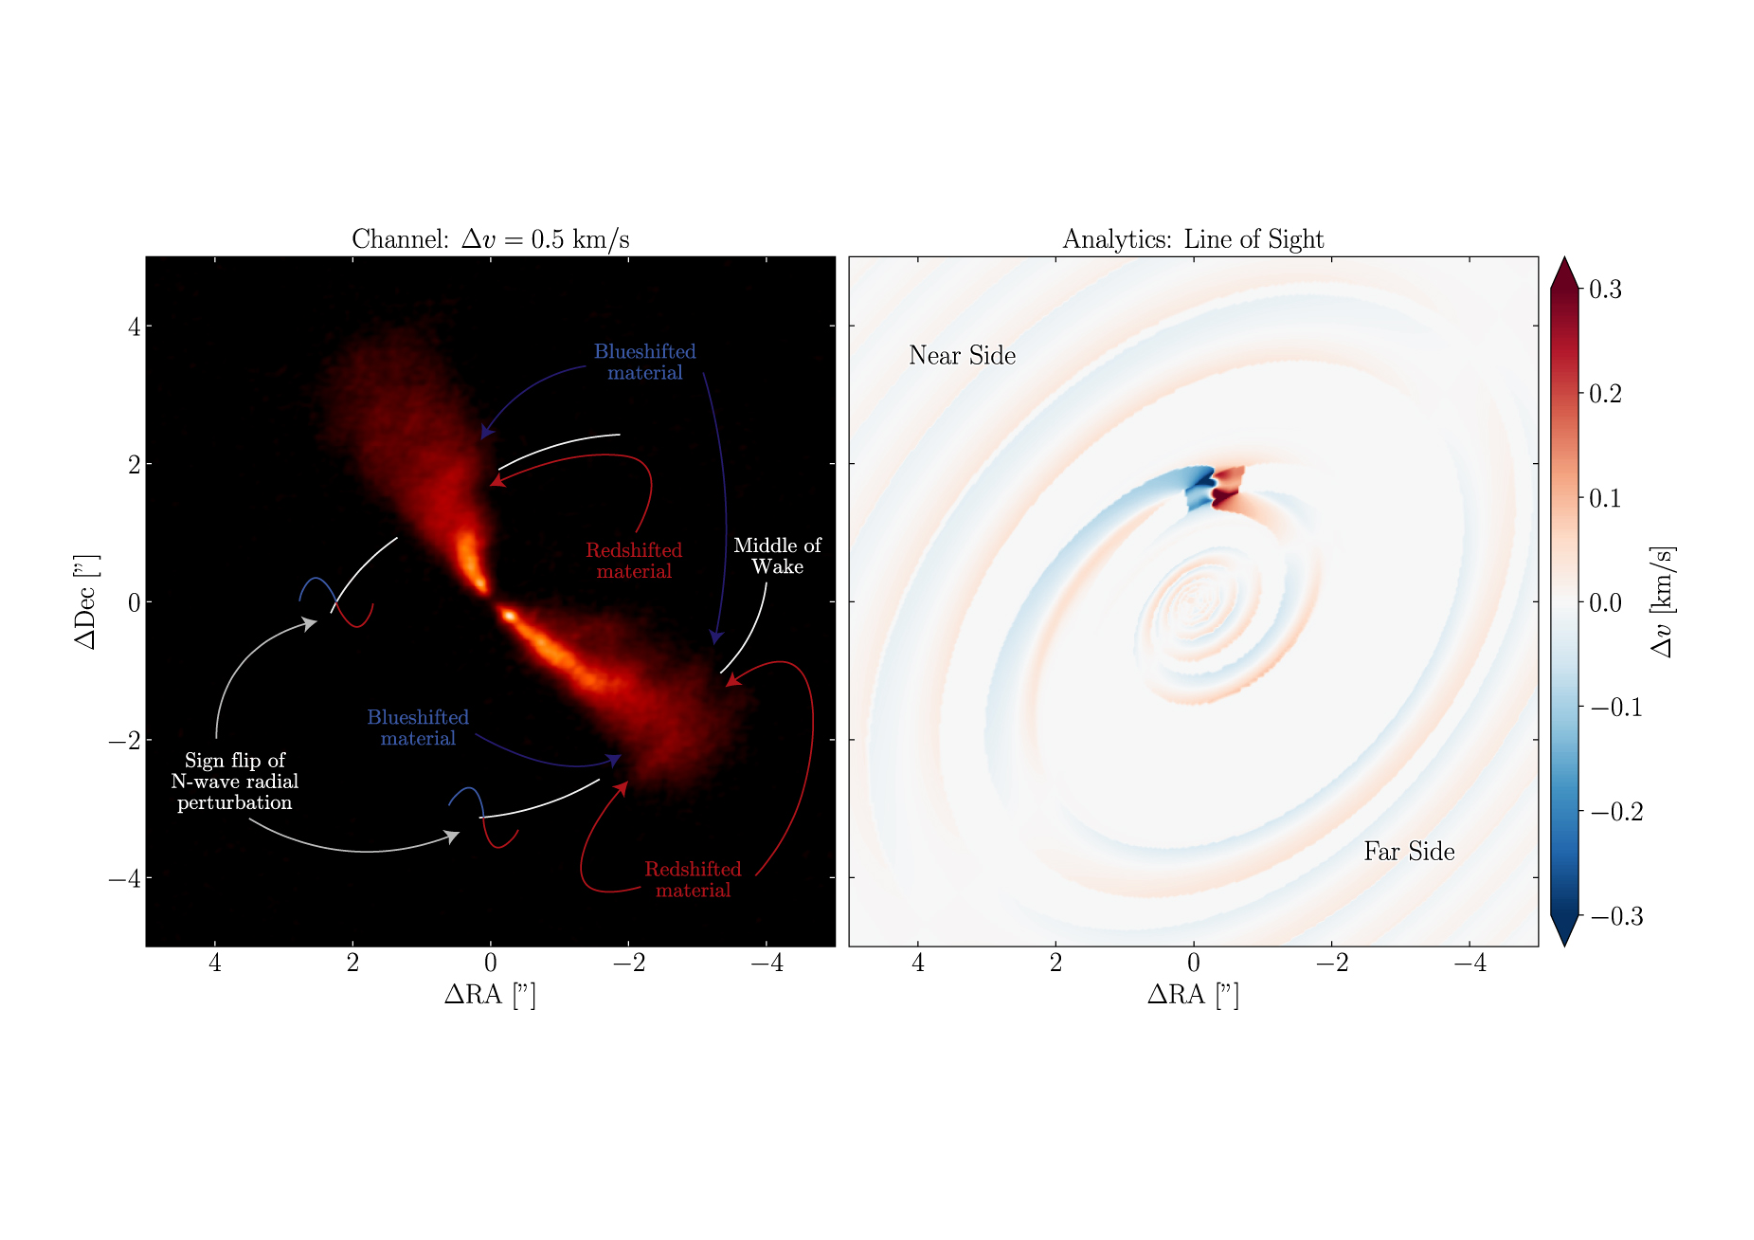
\includegraphics[width = 0.99\textwidth]{figures/calcino_channel_comparison.pdf}
    \caption{The left panel shows the $\Delta v = 0.5 \, \mathrm{km/s}$ velocity channel map of the line emission \citep{oberg2021}. The right panel shows the line-of-sight velocity perturbations from the semi-analytic model, projected to the emitting layer. Note that in both panels we define positive line-of-sight direction as away from the observer, while the negative direction is towards the observer. This yields the correct colour association with blue and redshift with the colourbar. Labels in the left panel indicate how the velocity kinks are associated with the blue and redshifting of velocities due to the planet wake crossing, as seen in the right panel. We also see a sign-flip in the perturbation in the channel across the semi-major axis, as expected for radial-dominated motions.}
    \label{fig:calcino_channel_comparison}
\end{figure}

Figure~\ref{fig:calcino_channel_comparison} shows the  $\Delta v = 0.2$ km/s channel in the left panel, and the line-of-sight velocity perturbations from the analytic model projected to the emitting surface in the right panel.
The annotations in the figure highlight how the perturbations from the wake shown in the right effect the channel.
Moreover the labels show how the perturbations change sign of the semi-major axis, which is as expected for perturbations dominated by radial motion.
While more subtle, the N-wave shape of the perturbation in the wake discussed in section~\ref{sec:asymptotic_N_wave} is also visible in the channel, especially on the south side (\citealt{rafikov2002a}, \citetalias{bollati2021}).

\begin{figure}
    \centering
    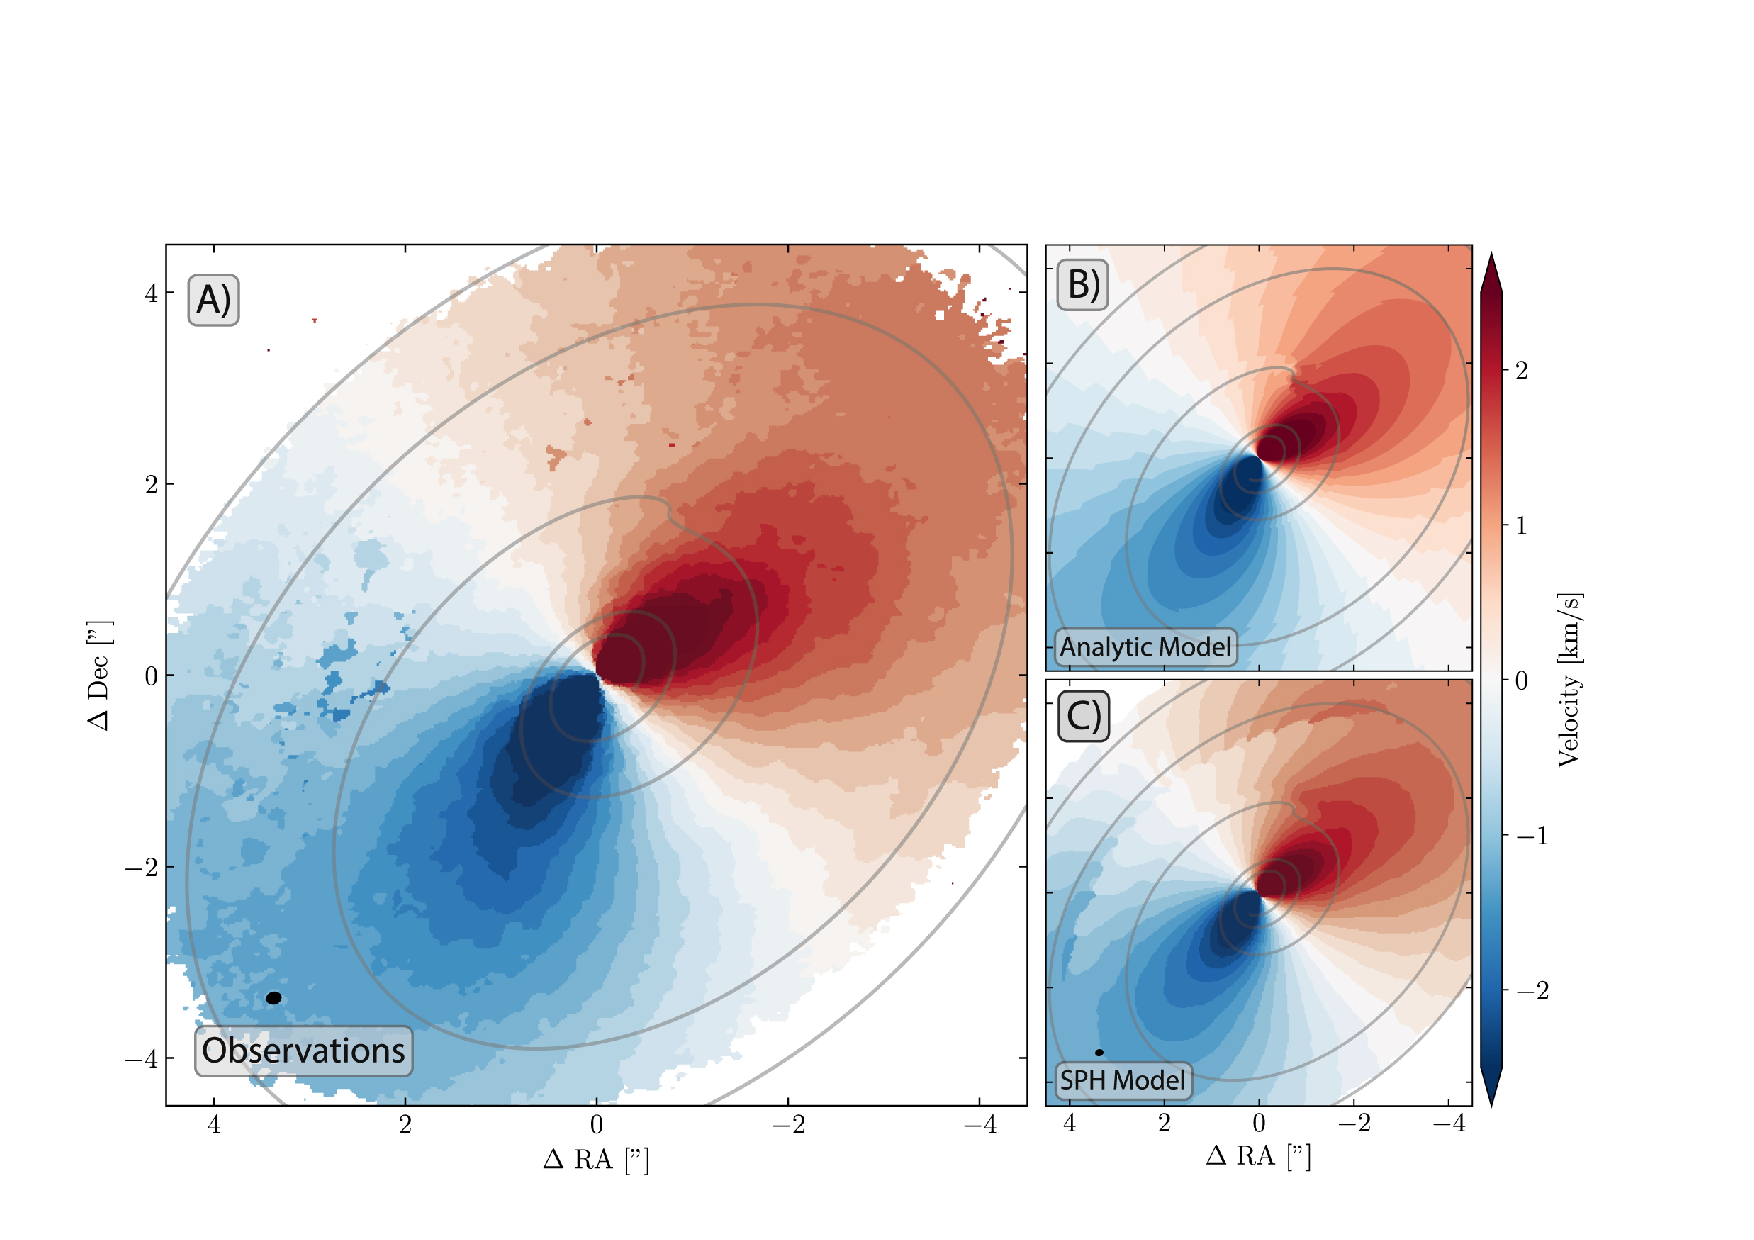
\includegraphics[width = 0.99\textwidth]{figures/calcino_v0.pdf}
    \caption{Panel A shows the peak velocity map of the HD~163296 disk from the line emission \citep{oberg2021}. The prediction from the semi-analytic and SPH + radiation transfer models are shown in panels B and C respectively. The projected wake as found from equation \ref{eq:power_law_wake} with $(H/r)_{\rm p}=0.08$ is shown in all panels. We see that in the models the wake traces spatially-correlated kinks across the entire disk. A similar tracing of features along the wake is seen in panel A, mapping the planet wake in the data.}
    \label{fig:calcino_v0}
\end{figure}

A comparison of the peak velocity map of HD~163296 between the observations, analytics, and SPH plus radiation transfer models are shown in Figure~\ref{fig:calcino_v0}.
The lines separating the coloured region of the contour plot are iso-velocity curves, and each of these roughly corresponds to the line of peak emission in a particular velocity channel.
Velocity kinks therefore show up in this plot as a ``wiggle'' in the iso-velocity curves, and so the planet wake causes deviations from the typical Keplerian butterfly planet expected for an unperturbed disk.
Plotted also is the projected wake shape, which we see traces the velocity kinks across successive lines of iso-velocity, revealing the planetary wake extended throughout the disk. 
The features are most visible along the semi-major axis, again suggesting radial-dominated perturbations.
They are additionally seen in both the analytic and SPH model.

%\begin{figure}
%    \centering
%    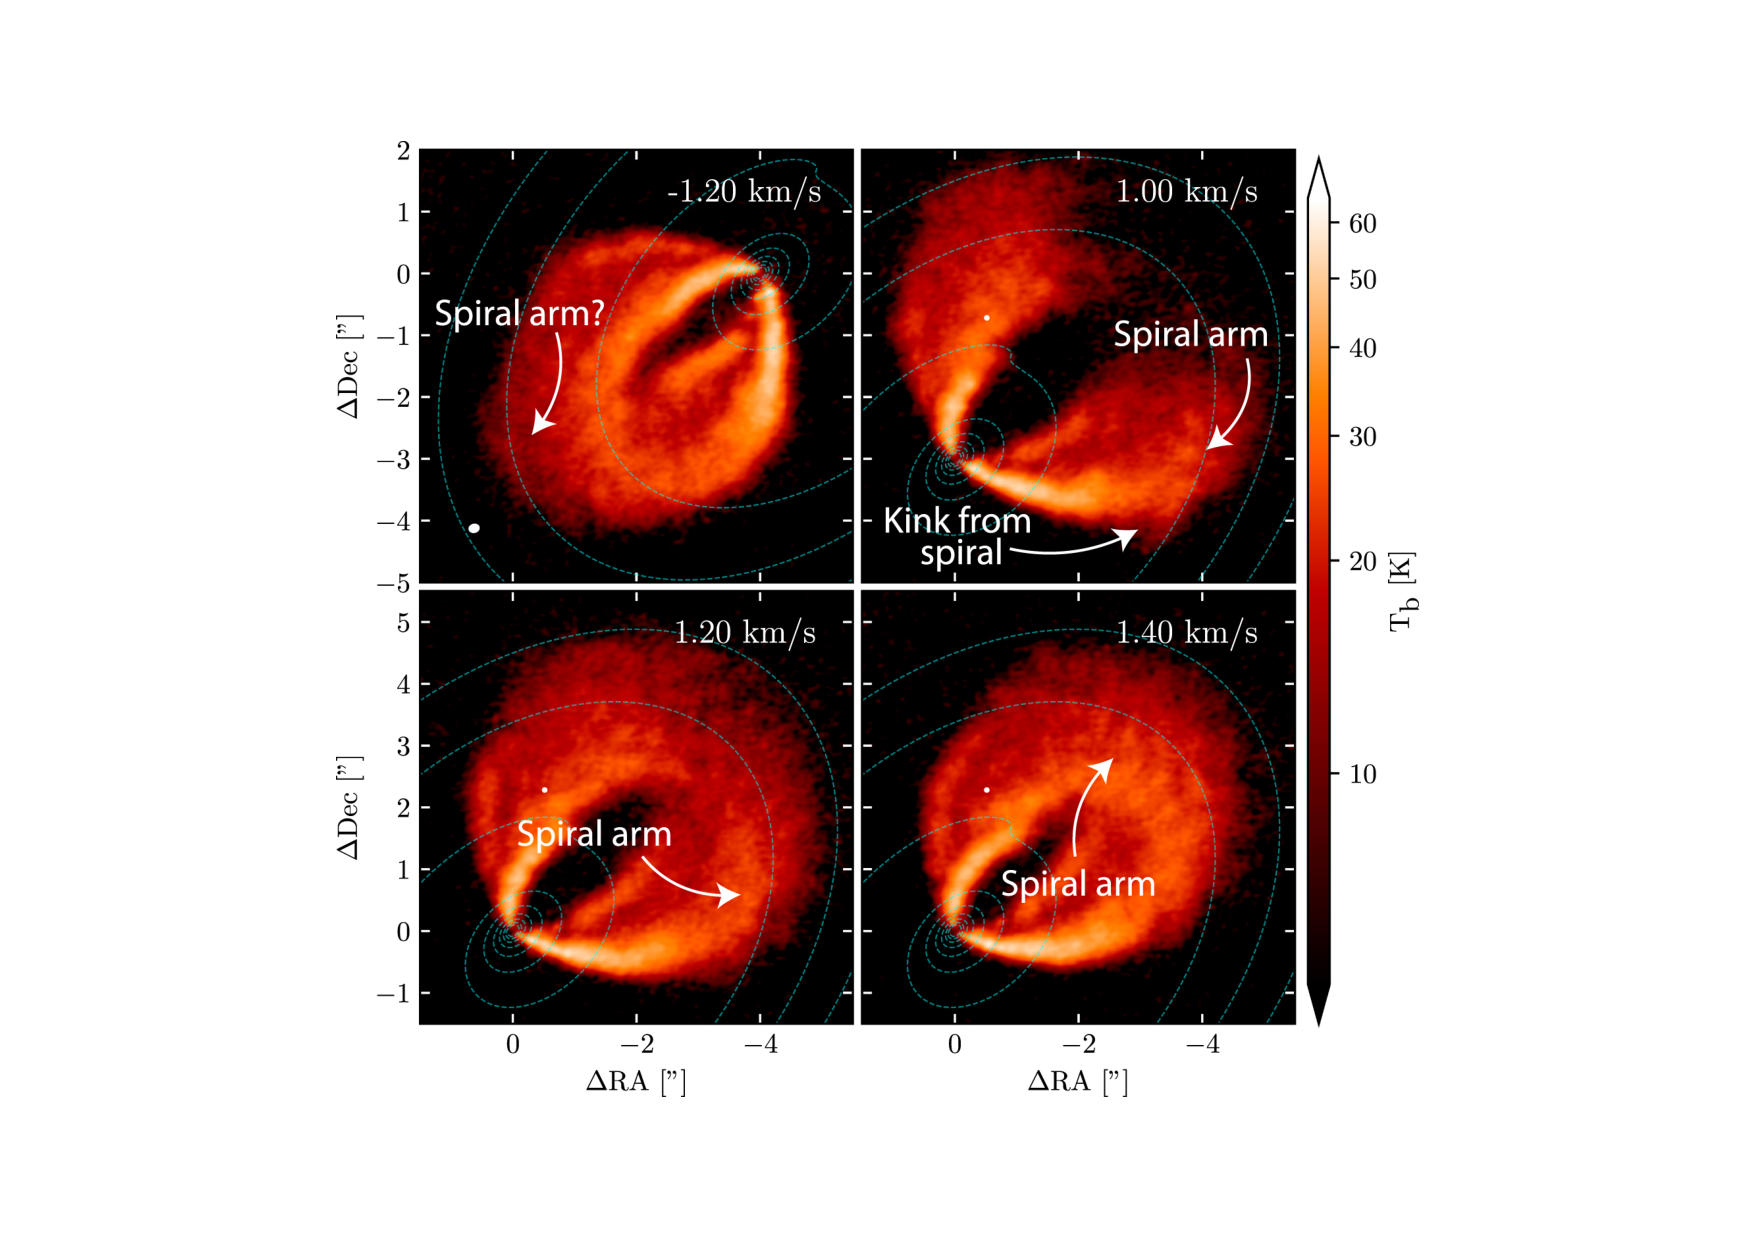
\includegraphics[width = 0.99\textwidth]{figures/calcino_shadows.pdf}
%    \caption{}
%    \label{fig:calcino_shadows}
%\end{figure}

%
%A final bonus is that the spiral arm is not just seen as velocity perturbations in the observations, but also in intensity.  Figure~\ref{fig:spiral} demonstrates this, showing selected channels from the data. Beginning with the top right panel, one may first observe the velocity kink associated with the spiral. The label indicates where the spiral arm can also be seen in intensity. The spiral continues in to the preceding channels in the bottom left and right panels. The spiral is co-located with the predicted location of the outer planet wake generated by the embedded protoplanet, as shown by the dotted cyan line.

\section{Discussion}

We have demonstrated:
\begin{enumerate}
    \item The spiral structures in HD~163296 reported by \citet{teague2021} are due to the planet wake induced by tidal-forcing of the embedded protoplanet \citep{pinte2018a}.
    \item The velocity damping proposed in \citetalias{bollati2021} is not necessary, as velocity kinks are indeed not localised to the planet location.
\end{enumerate}

These results also constitute the first direct confirmation of density waves generated by the Lindblad resonances in a circumstellar disk through the gravitational interaction of a planet.

\subsection{Density Waves or Buoyancy Spirals?}

Extended velocity perturbations associated with the embedded planet were also reported by \citet{teague2021} through calculating velocity residuals after subtracting a best-fitting flared Keplerian disk model.
They suggest that their results are evidence of buoyancy spirals \citep{zhu2012,bae2021}, since it was not previously believed that the Lindblad spiral could induce kinematic features far from the planet.
However the right panel of Figure~\ref{fig:calcino_channel_comparison} and Panel B of Figure~\ref{fig:calcino_v0} show that this is not the case, and that buoyancy spirals are not necessary to explain the observed secondary kinks \citepalias{bollati2021}.

Figure~\ref{fig:calcino_channel_comparison} provides strong evidence for the planet wake hypothesis over the buoyancy spirals hypothesis due to the obvious sign flip in the perturbations over the semi-major axis.
This is exactly as expected for the velocity perturbations in the planet wake, as they are dominated by radial motions as previously discussed.
As the name would suggest, buoyancy waves produce predominantly vertical motions \citep{bae2021}.
They therefore would not exhibit an abrupt sign change along the semi-major axis, or the semi-minor axis (which would be evidence of azimuthal perturbations).
It is also possible to look for the sign change more directly through velocity residual maps \citep{teague2021,izquierdo2021}, but we found that this easily confuses the resulting signs of each kinematic feature as the residuals are very sensitive to the background model subtracted.
Indeed, we found that even for simulations it is very challenging to correctly recover the sign of the perturbations accurately \citep[see Appendix~A of][for further detail]{calcino2022}.

We do also report additional kinematic structures (the opaque crosses in Figure~\ref{fig:calcino_channels}) that do not seem to be explained by the planet wake.
These features were also found by \citet{teague2021}, it is possible that they are the result of buoyancy spirals.
Their location is relatively consistent with this model, as buoyancy spirals excited by the planet have much smaller opening angles than the planet wake \citep{bae2021}.
Alternatively, the features could be due to the outer wake from a second embedded protoplanet orbiting at a smaller radius, as suggested by \citet{teague2018}.
Indeed \citep{pinte2020} reported a velocity kink located in the gap of the outermost ring seen in continuum, which they interpreted as evidence for an embedded planet.
Additional evidence for a kinematic planet signature in this region was found by \citet{teague2021}. 

\subsection{Estimating the Planet Mass}

Mapping the planet wake in HD~163296 suggests a powerful tool to aid in estimating the properties of both the embedded planet exciting the wake, and the protoplanetary disk itself.
\citetalias{bollati2021} showed that while the amplitude of generated velocity kinks is directly related to the mass of the perturbing body, the relevant unit of the planet mass (and so the kink amplitude) is the thermal mass \citep{goodman2001} given in equation \ref{eq:thermalmass}.
The thermal mass scales $M_{\rm th} \propto (H/r)_{\rm p}^3$ and so depends very sensitively on the temperature structure of the disk.
In order to measure the planet mass using disk kinematics, one must break the degeneracy between $M_{\rm p}$ and $(H/r)_{\rm p}$.

Constraints on the disk temperature may be found through measurements of CO emission \citep[e.g.][]{pinte2018},
but this does not determine either the mid-plane gas temperature or the scale height of the disk at the planet location, which is needed to constrain $M_{\rm th}$.
By assuming that the emission is optically thick, and thus $\mathrm{T_b}=\mathrm{T_{gas}}$, one may use the CO emission on both the upper and lower surfaces to determine the mid-plane temperature \citep{dullemond2020}.
The aforementioned assumption is however not guaranteed due to molecular freeze-out onto dust grains.
Mapping the spiral wake provides a natural way to measure the thermal mass directly and break the degeneracy.
From \ref{eq:power_law_wake} we can see that the way shape depends on the disk aspect ratio $(H/r)_{\rm p}$.
Thus, in principle it should be possible to measure the planet mass directly from kinematic observations by fitting both the amplitude of the kinks and the shape of the wake.
In practice this would require simultaneously fitting the kink amplitude, wake shape, emitting surface and density profile of the disk.
This is a complex procedure and so is beyond the scope of this Letter.
%
\subsection{Model Limitations} \label{sec:limitations}

The shape of the planet wake used here is calculated by integrating the Lin-Shu dispersion relation for a thin gas disk, and is derived under the tight-winding approximation (see section~\ref{sec:planetwake}).
It is therefore entirely linear \citep{ogilvie2002}, and so underestimates the pitch angle of spiral arms generated by planets exceeding the thermal mass (\citealt{zhu2015,bae2018a,cimerman2021}, \citeauthor{fasanoinprep.} in prep.).
\citet{cimerman2021} found that the non-linear propagation used in the semi-analytic models also over-predicts the decay rate of the density wave in the low mass regime, although this may not be the case for the high mass regime relevant here (\citeauthor{fasanoinprep.} in prep.).
The perturbation amplitude near the planet is also overestimated for planets over the thermal mass as already discussed (\citealt{goodman2001}, \citeauthor{fasanoinprep.} in prep.).
For this reason we used both analytical and SPH simulations, as the latter accounts for the global and fully non-linear behaviour of the solution.
From Figure~\ref{fig:calcino_v0} we see that the results are very similar in each case, suggesting that the problems with the semi-analytic models are limited when considering the observable aspects of the wake (at least for the parameters and especially the mass range tested here).

The simulated and analytic models both assume a locally isothermal temperature profile where the sound speed is independent of height in the disk.
However, HD~163296 is known to have a vertical temperature gradient \citep{rosenfeld2013,degregorio-monsalvo2013}, which should result in sound waves propagating faster in the higher and hotter layers of the disk.
This should result in an increased pitch angle for the planet wake in the upper layers \citep{juhasz2018}.
Vertical temperature gradients also allow for the excitation of buoyancy waves \citep{bae2021}.
From Figure~10 of \citet{law2021} we can see that the temperature gradient in the outer disk is very shallow up to multiple scale heights. 
Since this is the main region of concern here, temperature stratification is unlikely to have a large effect.

Finally, 3D wake propagation is known to deviate from the wake shape given in equation \ref{eq:power_law_wake}, even for relatively low mass planets.
\citet{zhu2015} found through numerical modelling that the spiral arms in a locally isothermal disk are more tightly wound in the upper layers.
The effect is captured in the SPH simulations we have performed, but not in the analytics nor in the wake shape projection.
It is interesting to note that this has the opposite effect to the temperature stratification, which should result in more open spirals.
Shock heating may also effect the evolution of the wake, and is not included in our simulations.
Treating the thermodynamics of the disk in more depth by calculating the temperature structure self-consistently and including shock heating would allow for these issues to be explored further, but is beyond the scope of this Letter.

\subsection{Summary}

We have demonstrated that the recently reported spiral structure in HD~163296 \citep{teague2021} is the outer planet wake generated by an embedded protoplanet \citep{pinte2018a}, providing the first confirmation of planetary wakes generated by the Lindblad resonances.

\section{The Planet Wake in IM Lupi} \label{sec:IMLupiwake}

This section presents part of \citet{verrios2022}, which is publicly available at \href{https://arxiv.org/abs/2207.02869}{\url{arXiv:2207.02869}}.

\subsection{Introduction}

The young star IM~Lupi is host to a large and spectacular circumstellar disk \citep{panic2009,avenhaus2018,cleeves2016,pinte2018}.
Localised deviations from Keplerian motion were found across multiple velocity channels in $^12$CO line emission observations \citep{pinte2020} taken as part of DSHARP \cite{huang2018,andrews2018}.
Higher spatial resolution observations from MAPS confirm the presence of these velocity kinks, which \citet{pinte2020} hypothesised to be induced by the gravitational disturbance from an embedded planet orbiting at $117$ au.
This separation is too large to facilitate the detection of such a planet through traditional methods like radial velocities or transits, and the optically thick dust and gas material complicates direct imaging.

Scattered light images of the disk reveal large, tightly-wound spiral structures in the disk surface \citep[see Figure~\ref{fig:im_lup};][]{avenhaus2018},
while 1.25 mm continuum observations from DSHARP show also spiral arms and gaps in the dust-disk present in the mid-plane (see row 2 panel 1 of Figure~\ref{fig:maps_disks}; \citealt{huang2018}).
Are these spirals caused by the embedded protoplanet?
An alternative explanation if that they are formed through gravitational instabilities, which produce disordered flocculuent spirals and hence ``kinks everywhere'' \citep{hall2020}.
On the other hand, planets should produce velocity kinks only along the coherent one-armed planet wake.
The gravitational instability requires that the disk is self-gravitating and so massive, which is not required by the planet model.

In this letter we investigated whether an embedded planet can produce both the observed spiral structures and the observed kinematic features.
Here, we present the portion of the letter concerned with tracing the planet wake in the kinematics, similarly to in \citet{calcino2022}.

\subsection{Simulated Model}

We used the \textsc{phantom} SPH code \citep{price2018} to create models of the interaction between the disk of IM Lupi and an embedded planet.
A disk of mass $0.01 \, \mathrm{M_\odot}$ was modelled using ten million SPH particles, set to initially follow the density profile given in equation~\ref{eq:sigma_phantom}.
We used $p=0.48$ \citep{pinte2018} and $r_{\rm c}=150$ au.
We assumed a locally isothermal equation of state with $c \propto r^{-0.31}$, and a disk aspect ratio of $H/r=0.129$ at $r=100$ au.
The central star was modelled as a sink particle \citep{bate1995}, with a mass of $1.12 \, \mathrm{M_\odot}$ \citep{andrews2018} and an accretion radius of $1$ au.
We included dust in the simulations using the \textsc{multigrain} one-fluid algorithm \citep{price2015,ballabio2018,hutchison2018,price2018}.
We used 11 distinct grain sizes, logarithmically spaced between $a_{\rm min}=1.0 \, \mathrm{\mu m}$ and $a_{\rm max}=2300 \, \mathrm{\mu m}$ and following a distribution given by $dn(a) \propto a^{-3.5} \, da$.
The gas to dust ratio was set as $57$ resulting in a total dust mass of $1.7 \times 10^{-3} \, \mathrm{M_\odot}$ following \citep{pinte2018}. 

The planet was modelled as a non-accreting sink particle with a softened gravitational potential, following a procedure similar to that in \citet{szulagyi2016}.
This was done to minimise the fast migration and large mass growth that an accreting particle would experience due to the large number of SPH particles.
We performed simulations with varying planet masses of $2, \, 3, \, 5$ and $7\, \mathrm{M_J}$, although we will only discuss the $2 \, \mathrm{M_J}$ model here.

Radiation transfer was then performed on the SPH models using \textsc{mcfost} \citep{pinte2006,pinte2009} following a similar method to that outlined in sections~\ref{sec:garg_analytics} and \ref{sec:calcino_hydro}.
Refer to \citet{verrios2022} for further detail.

\subsection{Tracing the Wake}

\begin{figure}
    \centering
    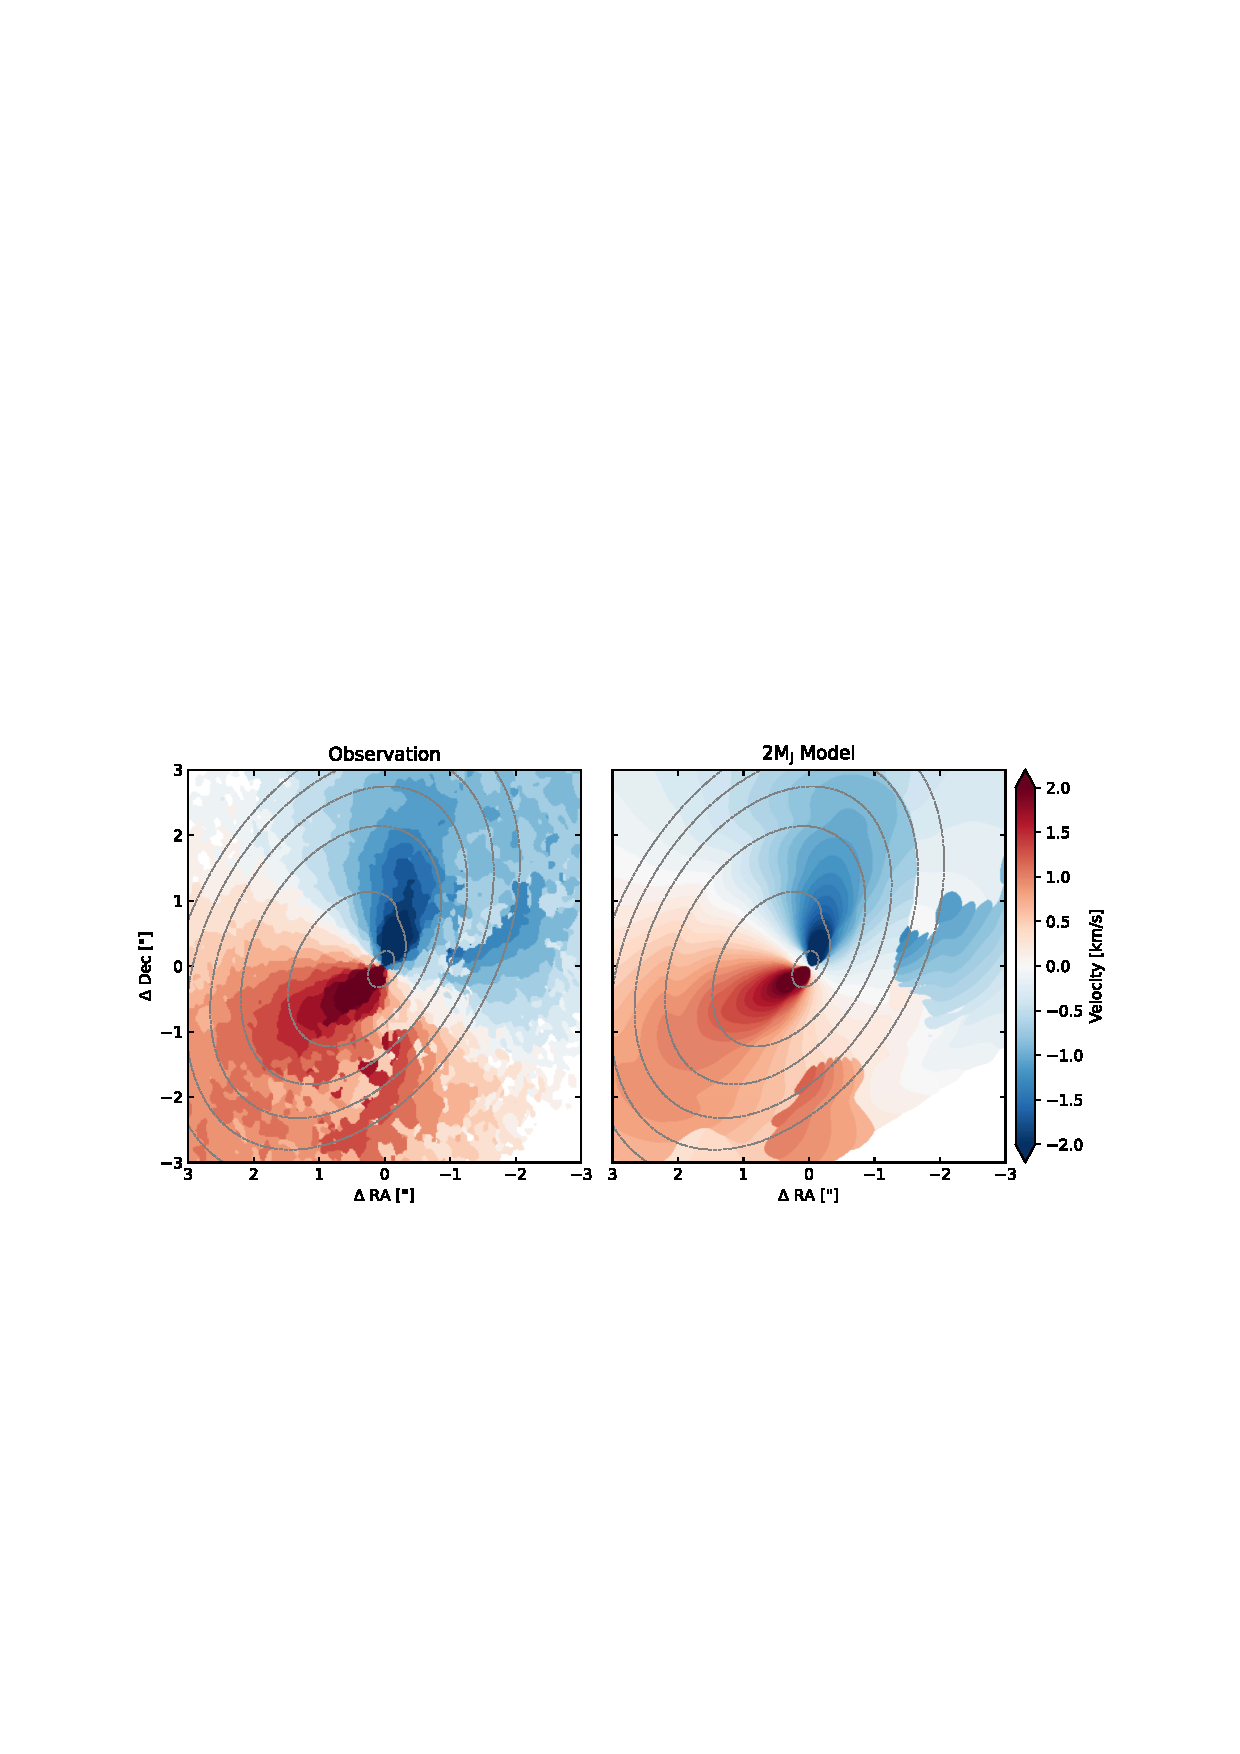
\includegraphics[width = 0.99\textwidth]{figures/verrios_v0.pdf}
    \caption{The left panel shows the peak velocity map of the $^{12}$CO line emission data from MAPS \citep{oberg2021}. The right panel shows the analogous synthetic map produced with our $2 \, \mathrm{M_J}$ model. The dotted line in both panels shows the expected location of the planet wake as predicted by linear theory \citep{ogilvie2002}, projected to the top emitting surface of the disk \citep{pinte2018,law2021}.}
    \label{fig:verrios_v0}
\end{figure}

A key prediction of the embedded planet hypothesis is that the one-armed planet wake excited by the planet should create velocity kinks any time it spatially crosses a channel.
\citet{calcino2022} found that this may be used to trace the planet wake shape through kinematic observations.
The presence of a coherent planet wake in the observations would provide evidence for the embedded planet model over gravitational instability.
\citet{calcino2022} also found that the wake is best traced in the peak velocity map.

Were therefore use spectrally collapsed both the MAPS $^{12}$CO observations \citep{oberg2021} and the synthetic observations from our SPH + radiation transfer model to create peak velocity maps.
These are plotted in Figure~\ref{fig:verrios_v0}, with the data shown in the left panel, and the model in the right.
We additionally calculated the expected wake shape using \ref{eq:power_law_wake} \citep{ogilvie2002,rafikov2002a}, and projected it to the emission surface determined by \citet{law2021a} following the method of \citet{calcino2022}.
This is shown in both panels (grey dashed line).
The velocity perturbations, which manifest as distorted contours, are seen to trace the planet wake shape through the outer disk in both the model and the observations.
The are particularly obvious in the second passage of the outer wake in the north side of the disk.
In addition, the ``N-wave'' structure predicted by the semi-analytic models (\citealt{goodman2001}; \citealt{rafikov2002a}; \citetalias{bollati2021}) can be seen in the observations in that same region.

We therefore confirm that the wake from the planet is visible in the peak velocity map of the $^{12}$CO observations, as predicted by the embedded planet model.




%The distorted contours in the observational data appear to follow the planet wake both inside and outside the planet location, particularly in the second spiral. Particularly intriguing is the “N-wave” structure apparent in the distorted contours around the dashed line in the observational map, which are predicted by both our simulations (right panel) and by semianalytic models of planet wake propagation (Rafikov 2002; Bollati et al. 2021).